%%
%% CoEvoP&R ASP-DAC 2027 manuscript skeleton.
%%
\PassOptionsToPackage{table}{xcolor}
\documentclass[sigconf,anonymous,review]{acmart}

\usepackage{algorithm}
\usepackage{algorithmic}
\usepackage{multirow}
\usepackage{caption}
\captionsetup{font=small}
\definecolor{rankfirst}{HTML}{FFCCCC}
\definecolor{ranksecond}{HTML}{CCE5FF}

\AtBeginDocument{%
  \providecommand\BibTeX{{%
    Bib\TeX}}}

%% ASP-DAC 2027 initial submissions are double-blind. CCS metadata can be
%% restored for the camera-ready version if ACM/ASP-DAC requires it.
\settopmatter{printccs=false}

\setcopyright{none}
\copyrightyear{2027}
\acmYear{2027}
%% TODO(camera-ready): ACM assigns the DOI after acceptance and copyright transfer.
\acmDOI{}
\acmConference[ASPDAC '27]{32nd Asia and South Pacific Design Automation Conference
  (ASP-DAC 2027)}{January 25--28, 2027}{Tokyo, Japan}
\acmBooktitle{Proceedings of the 32nd Asia and South Pacific Design Automation
  Conference (ASP-DAC 2027), January 25--28, 2027, Tokyo, Japan}
%% TODO(camera-ready): ACM assigns the ISBN after acceptance and copyright transfer.
\acmISBN{}

\begin{document}

\title{CoEvoP\&R: Co-Evolving Placement Objectives with Routing Feedback via Large Language Models}

%% Initial review is anonymous. Replace these placeholders for camera-ready.
\author{Anonymous Author(s)}
\affiliation{%
  \institution{Anonymous Institution}
  \country{Anonymous Country}}

\renewcommand{\shortauthors}{Anonymous}

\begin{abstract}
Analytical placers optimize half-perimeter wirelength (HPWL) and density, but
recent post-route benchmarking studies show that these proxies correlate poorly with
routed wirelength, routing congestion, and timing. Existing routing-aware placers
handle this gap with fixed expert terms or learned black-box surrogates, leaving
the differentiable objective itself fixed. CoEvoP\&R instead makes complete
replacement objectives the search target. A large language model (LLM)
proposes readable symbolic programs, DREAMPlace measures their optimizer
behavior, and scheduled routed promotions condition later proposals.
This optimizer-embedded loop requires every candidate to pass a restricted
objective interface, autograd checks, term-compatibility rules, and a
cost-scaled placement/routing cascade. A perturbation-based proxy audit gives
cheap timing proxies selection influence only when they are non-redundant with
HPWL and agree with downstream timing. CoEvoP\&R is evaluated on ChiPBench Nangate45, ICCAD
2015 Superblue, and ASAP7 cross-node transfer. On the primary ChiPBench
benchmark, CoEvoP\&R reduces DREAMPlace HPWL by 16.9\% and density overflow
by 36.7\% on average over native DREAMPlace, while improving OpenTimer
placement-RC WNS by 0.70 ns and TNS by 912 ns. Each search returns a compact
symbolic objective that plugs directly into DREAMPlace.
\end{abstract}

\begin{CCSXML}
<ccs2012>
<concept>
<concept_id>10010147.10010178.10010179</concept_id>
<concept_desc>Computing methodologies~Machine learning</concept_desc>
<concept_significance>500</concept_significance>
</concept>
<concept>
<concept_id>10010583.10010786</concept_id>
<concept_desc>Hardware~Electronic design automation</concept_desc>
<concept_significance>500</concept_significance>
</concept>
<concept>
<concept_id>10010583.10010588.10010559</concept_id>
<concept_desc>Hardware~Physical design (EDA)</concept_desc>
<concept_significance>500</concept_significance>
</concept>
</ccs2012>
\end{CCSXML}

\ccsdesc[500]{Computing methodologies~Machine learning}
\ccsdesc[500]{Hardware~Electronic design automation}
\ccsdesc[500]{Hardware~Physical design (EDA)}

\keywords{electronic design automation, placement, routing, large language models,
  objective functions}

\maketitle

% Queue the two-column method overview before page 2 begins.
\begin{figure*}[!t]
\centering
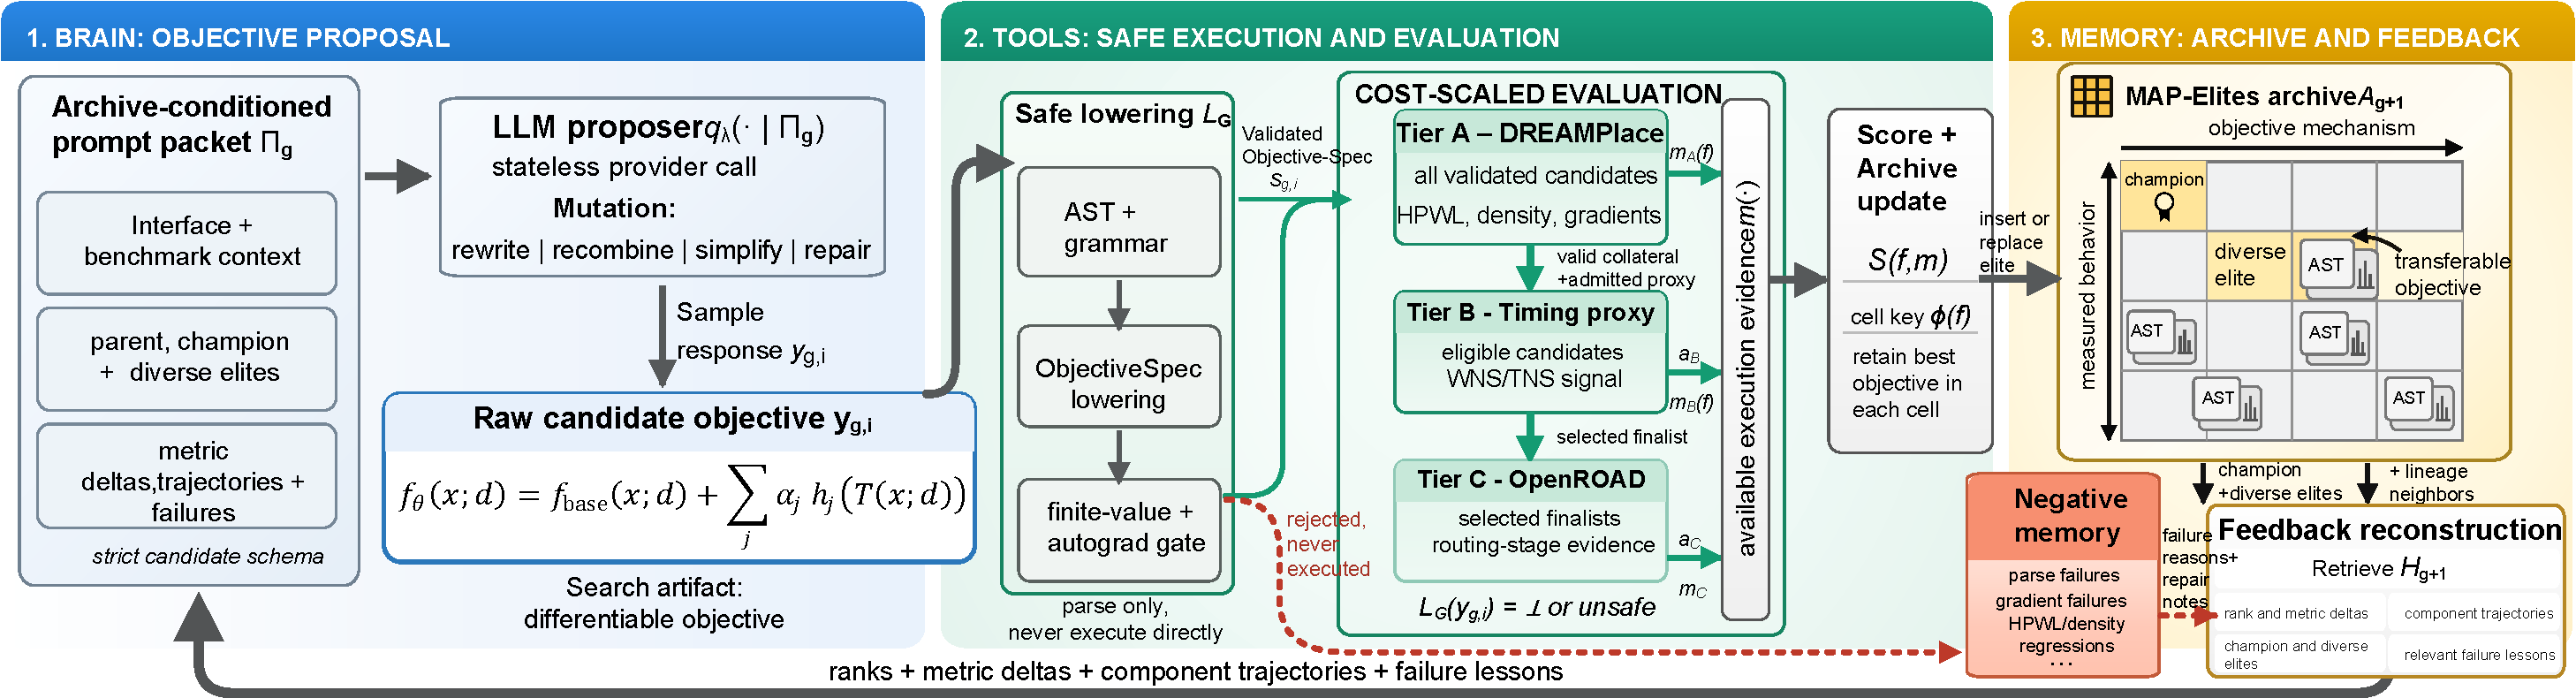
\includegraphics[width=\textwidth]{graphs/Figure1.pdf}
\caption{CoEvoP\&R evolves complete placement objectives through
archive-conditioned proposal, safe EDA evaluation, and scheduled routed
feedback.}
\Description{An LLM proposes objective programs, a restricted interface lowers
and evaluates them with EDA tools, and an archive reconstructs measured
feedback for later proposals.}
\label{fig:loop}
\end{figure*}

\section{Introduction}

Modern analytical placers make global placement tractable by optimizing
half-perimeter wirelength (HPWL) plus a density penalty. These cheap, smooth
proxies enable gradient-based tools such as DREAMPlace~\cite{dreamplace}.
However, the same objective choice also limits
what the placer can optimize. ChiPBench shows that placement-stage HPWL
correlates poorly with post-route quality on modern industrial designs,
including routed wirelength, routing congestion, worst negative slack (WNS),
total negative slack (TNS), and design-rule checking (DRC)
count~\cite{chipbench}. The analytical placer optimizes one target while the
completed flow depends on another.

Routing-aware placement has addressed this mismatch through two main changes
to the objective. The first adds hand-engineered symbolic terms on top of a
fixed placement objective. Rectangular Uniform wire DensitY (RUDY) estimates
routing demand from placement geometry~\cite{rudy}, and later congestion and
density controls build on the same idea. Terms of this kind sharpen routing
awareness but fix the objective form and require expert redesign for each
technology or benchmark family. The second inserts learned routing or timing
surrogates into placement. LaMPlace improves post-route WNS by 43.0 percent
and TNS by 30.4 percent~\cite{lamplace}. GOALPlace reduces DRC violations by
up to tenfold~\cite{goalplace}. RoutePlacer lowers routing congestion while
preserving routed wirelength~\cite{routeplacer}. These methods add downstream
awareness but embed part of the objective in black-box models that engineers
cannot inspect or edit. Neither change makes the differentiable placement
objective itself searchable. This leaves an open third path: direct search over
readable, differentiable objective forms that still run inside analytical
placement.

CoEvoP\&R searches this third path with LLM program evolution. FunSearch,
Eureka, LLM-SR, and AlphaEvolve show that LLMs can revise executable programs
using automatic evaluator feedback~\cite{funsearch,eureka,llmsr,alphaevolve}.
EvoPlace and VeoPlace bring foundation-model search into placement by evolving
optimizer components or guiding macro-placement
actions~\cite{evoplace,veoplace}. These systems search initialization,
optimizer, or action choices around the analytical objective. CoEvoP\&R
searches the objective itself: an LLM proposes complete symbolic replacement objectives,
and DREAMPlace evaluates each safe candidate inside the gradient path that
produces a placement. This embedding makes optimizer
compatibility part of the search space. Static admission, diagnostic autograd
checks, and runtime guards reject incompatible or unstable objectives. Because
full OpenROAD routing is too expensive for every candidate, scheduled
promotions return routed evidence to later proposals~\cite{openroad}. A proxy
audit gives cheap timing signals selection influence only after they are
non-redundant with HPWL and agree with downstream timing.

CoEvoP\&R makes four contributions.
\begin{itemize}
  \item \textbf{Searchable objectives.} CoEvoP\&R searches complete
  differentiable replacement objectives and discovers readable formulas that
  improve placement and post-GRT quality over the native DREAMPlace objective.
  \item \textbf{Optimizer-embedded evolution.} CoEvoP\&R inserts each LLM
  objective into the DREAMPlace gradient path through static, diagnostic, and
  runtime safety checks.
  \item \textbf{Proxy audit.} CoEvoP\&R gives cheap timing proxies
  selection influence only after non-redundancy and routed-agreement checks.
  \item \textbf{Deployable artifact.} Each CoEvoP\&R search returns a compact
  symbolic objective that engineers can inspect, edit, and plug into DREAMPlace.
\end{itemize}

On the primary Nangate45 panel, CoEvoP\&R reduces DREAMPlace HPWL by 16.9\%
and density overflow by 36.7\% on average, while improving OpenTimer
placement-RC WNS by 0.70 ns and TNS by 912 ns.


\section{Related Work}

\paragraph{Routability-Aware Objectives.}
Routability-aware placement exposes downstream routing or timing cost to an
analytical optimizer. RePlAce established the electrostatic density
formulation~\cite{replace}, and DREAMPlace made analytical placement
GPU-efficient in PyTorch~\cite{dreamplace}. One line adds expert symbolic
terms: RUDY estimates routing demand from placement
geometry~\cite{rudy}. A second line inserts learned downstream surrogates.
LaMPlace, GOALPlace, and RoutePlacer connect placement to post-route timing,
design-rule checking (DRC), or congestion through masks, graph neural
networks, and learned routability signals~\cite{lamplace,goalplace,routeplacer}.
These methods add downstream awareness through fixed expert terms or learned
components. CoEvoP\&R searches for readable symbolic objective forms that
still execute inside the analytical placer.

\paragraph{Foundation-Model Placement Search.}
Placement search methods differ by the artifact they modify. Reinforcement
learning places macros sequentially~\cite{mirhoseini2021}. AutoDMP tunes
macro-placement parameters with multi-objective Bayesian
optimization~\cite{autodmp}, and HyperPlace uses an off-the-shelf LLM to tune
GPU-placer hyperparameters~\cite{hyperplace}. EvoPlace evolves optimizer
code, including initialization, preconditioning, and update components, with
HPWL feedback~\cite{evoplace}. VeoPlace uses a vision-language model (VLM) to
guide macro-placement actions through evolutionary search~\cite{veoplace}.
ChiPBench provides end-to-end validation for whether
placement gains survive downstream flow~\cite{chipbench}. These systems
search parameters, optimizer components, or macro actions around the placement
objective. CoEvoP\&R targets the differentiable objective itself and uses
scheduled routed promotions to condition later objective proposals.

\paragraph{Executable LLMs for EDA.}
LLM-based EDA work often uses models for text, register-transfer level (RTL),
or prediction tasks. ChipNeMo adapts foundation models for chip-design
tasks~\cite{chipnemo}. RTLCoder generates Verilog from natural
language~\cite{rtlcoder}. MasterRTL and VeriLoC predict pre-synthesis power,
performance, area, or line-level design quality from
Verilog~\cite{masterrtl,veriloc}. A second line turns LLM output into
executable programs. FunSearch searches over Python programs for
combinatorial mathematics~\cite{funsearch}. Eureka evolves reward functions
from training-statistics feedback~\cite{eureka}. Evolution of Heuristics
(EoH) co-evolves natural-language thoughts and executable heuristic
code~\cite{eoh}. LLM-SR recovers symbolic scientific equations under
automated evaluation~\cite{llmsr}. AlphaEvolve extends the pattern to full
code files across mathematics and computing infrastructure~\cite{alphaevolve},
and OpenEvolve provides a public implementation~\cite{openevolve}. These
systems evaluate generated programs after execution. CoEvoP\&R places
generated code inside DREAMPlace's autograd path, so validity requires finite
objective values, finite gradients, and optimizer-compatible terms before
routed validation.


\section{Method}

CoEvoP\&R searches the differentiable placement objective while keeping
DREAMPlace's optimizer fixed. This isolates objective quality and permits new
interactions among wirelength, density, routing pressure, and timing-relevant
observables that fixed-form parameter tuning cannot express.
Figure~\ref{fig:loop} shows the loop: archive-conditioned proposal, restricted
lowering, cost-scaled EDA evaluation, and feedback reconstruction. The LLM
neither invokes the EDA tools nor selects fitness.

\subsection{Problem Formulation}
\label{sec:problem}

Let $d\in\mathcal{D}$ denote a design, $s$ a placement seed, and
$\mathbf{x}$ the positions of all movable macros and standard cells. A
candidate objective $f$ produces the mixed-size placement
\begin{equation}
\mathbf{x}_{d,s}(f)=\mathcal{P}_{d,s}(f),
\label{eq:placement-map}
\end{equation}
where $\mathcal{P}_{d,s}$ is DREAMPlace with its native objective replaced by
$f$; the optimizer and downstream evaluators remain fixed.

Let $\mathcal{T}=\{t_1,\ldots,t_k\}$ contain the allowed differentiable
observables. The first call records each term scale $\kappa_j$, which remains
fixed for the run. A complete replacement objective is
\begin{equation}
\widetilde t_j(\mathbf{x};d)=
\frac{t_j(\mathbf{x};d)}{\kappa_j},\qquad
f_\theta(\mathbf{x};d)=\kappa_{\mathrm{wl}}
F_\theta\!\left(\widetilde{\mathcal{T}}(\mathbf{x};d)\right),
\label{eq:candidate-objective}
\end{equation}
where restricted program $F_\theta$ has one wirelength and one density anchor;
routing terms and nonlinear interactions are optional.
$\kappa_{\mathrm{wl}}$ restores wirelength scale. The expression, constants,
term set, and named diagnostics form its lowered \texttt{ObjectiveSpec}.
Equation~\eqref{eq:candidate-objective} defines the entire minimized objective,
not a residual around a hidden native loss.

For evaluator $E_j$, define
$m_j(f;d,s)=E_j(\mathbf{x}_{d,s}(f))$ and let $f_0$ denote native
DREAMPlace. CoEvoP\&R orients every metric so that positive gain is better:
\begin{equation}
g_j(f;d,s)=o_j\,
\frac{m_j(f;d,s)-m_j(f_0;d,s)}{\nu_j},
\quad o_j\in\{-1,+1\},
\label{eq:metric-gain}
\end{equation}
where $o_j=-1$ for costs, $o_j=+1$ for WNS and TNS, and $\nu_j>0$ is a
fixed panel-specific scale. Density overflow measures placement feasibility;
routing congestion and routed wirelength come only from the routed evaluator.

Search-panel evidence guides parent selection; final-panel metrics never enter
prompts or archive fitness. Budgets $B_A,B_B,B_C$ bound placement, timing, and
routing calls. Selection of the returned objective is restricted to candidates
with Tier-C evidence:
\begin{equation}
f^*=\arg\max_{f\in\mathcal{A}^{C}_G}S_{\mathrm{final}}(f),
\quad N_\ell\leq B_\ell,\ \ell\in\{A,B,C\},
\label{eq:routed-objective}
\end{equation}
where $\mathcal{A}^{C}_G$ is the routed subset of the final archive. Thus,
search guidance and final evidence remain disjoint.

\subsection{Archive-Conditioned Proposal}
\label{sec:proposer}

Evolution starts from a measured portfolio of native-equivalent, alternative
wirelength-density, density-heavy, and routing-aware formulas. Valid symbolic
seeds populate the islands of $\mathcal{A}_0$; native DREAMPlace remains an
external, uneditable reference. Each island receives a measured eligible seed
before LLM sampling.

The controller rotates across islands and samples a parent from the current
island's eligible MAP-Elites cells. Let $S_A(p)$ be the constrained Tier-A
score defined below, $d_{\mathrm{base}}(p)\in[0,1]$ the distance from the
nearest fixed mechanism, and $n_g(\mathrm{sig}(p))$ the number of candidates
with the same mechanism signature. The implemented novelty-aware distribution
is
\begin{equation}
\begin{aligned}
\pi_{\mathrm{par}}(p\mid\mathcal{A}_g)
&=\frac{w_g(p)}{\sum_{u\in\mathcal{P}_g}w_g(u)},\\
w_g(p)&=\max\{\log(1+[S_A(p)]_+),\epsilon\}\\
&\quad\times\frac{\tfrac12+d_{\mathrm{base}}(p)}
{\sqrt{n_g(\mathrm{sig}(p))}}.
\end{aligned}
\label{eq:parent-policy}
\end{equation}
for $p$ in parent pool $\mathcal{P}_g$, which contains admitted elites and
bounded, behaviorally distinct near misses but excludes structural failures
and severe regressions. The mechanism-count denominator prevents repeated
sampling of one family.

The prompt never contains the full archive. Retrieval constructs
\begin{equation}
\begin{aligned}
\mathcal{H}_g={}&\{f_0,p_g\}\cup\operatorname{Top}(\mathcal{A}_g)
\cup\operatorname{Diverse}(\mathcal{A}_g,\phi)\\
&\cup\operatorname{NearMiss}(\mathcal{A}_g)
\cup\operatorname{RelevantFail}(\mathcal{A}_g,p_g).
\end{aligned}
\label{eq:retrieval-policy}
\end{equation}
The bounded sets provide a champion, high scorers, behaviorally diverse cells,
useful tradeoffs, and failures relevant to the selected parent's terms.
Duplicate programs are removed unless measured outcomes differ. The controller
then builds
\begin{equation}
\Pi_g=\bigl(\underbrace{r,\iota,b,\sigma}_{\text{fixed contract}},
\underbrace{p_g,u_g,\mathbf{m}_g,\mathcal{H}_g}_{\text{measured context}}\bigr),
\label{eq:prompt-packet}
\end{equation}
where $(r,\iota,b,\sigma)$ fixes the task, objective API, target context, and
JSON schema. Adaptive fields supply the parent, edit mode, evaluator scorecard,
and retrieved programs. Gate thresholds remain hidden so that proposals use
measured behavior rather than copy admission rules.

The controller normally requests a SEARCH/REPLACE edit and switches to a full
rewrite after repeated static rejection. A stateless provider produces $K$
independent responses from the same packet:
\begin{equation}
\mathcal{S}_g=\left\{L_{\mathcal{G}}(y_{g,i})\mid
y_{g,i}\sim q_\lambda(\cdot\mid\Pi_g),\;
L_{\mathcal{G}}(y_{g,i})\neq\bot\right\}_{i=1}^{K}.
\label{eq:candidate-set}
\end{equation}
Each response contains \texttt{id}, \texttt{rationale},
\texttt{parent\_ids},
\texttt{declared\_\allowbreak term\_\allowbreak usage},
\texttt{change\_\allowbreak description}, and a complete
\texttt{objective\_\allowbreak program}. Provider retries repair malformed or rejected
responses within the same sample. Deterministic coefficient siblings calibrate
accepted routing mechanisms; they share one lineage, but each consumes
evaluator budget.

Figure~\ref{fig:prompt-schema} exposes the proposal and lowering contracts.
It also distinguishes independent samples from retries and generated code from
the executable record.

\begin{figure}[t]
\centering
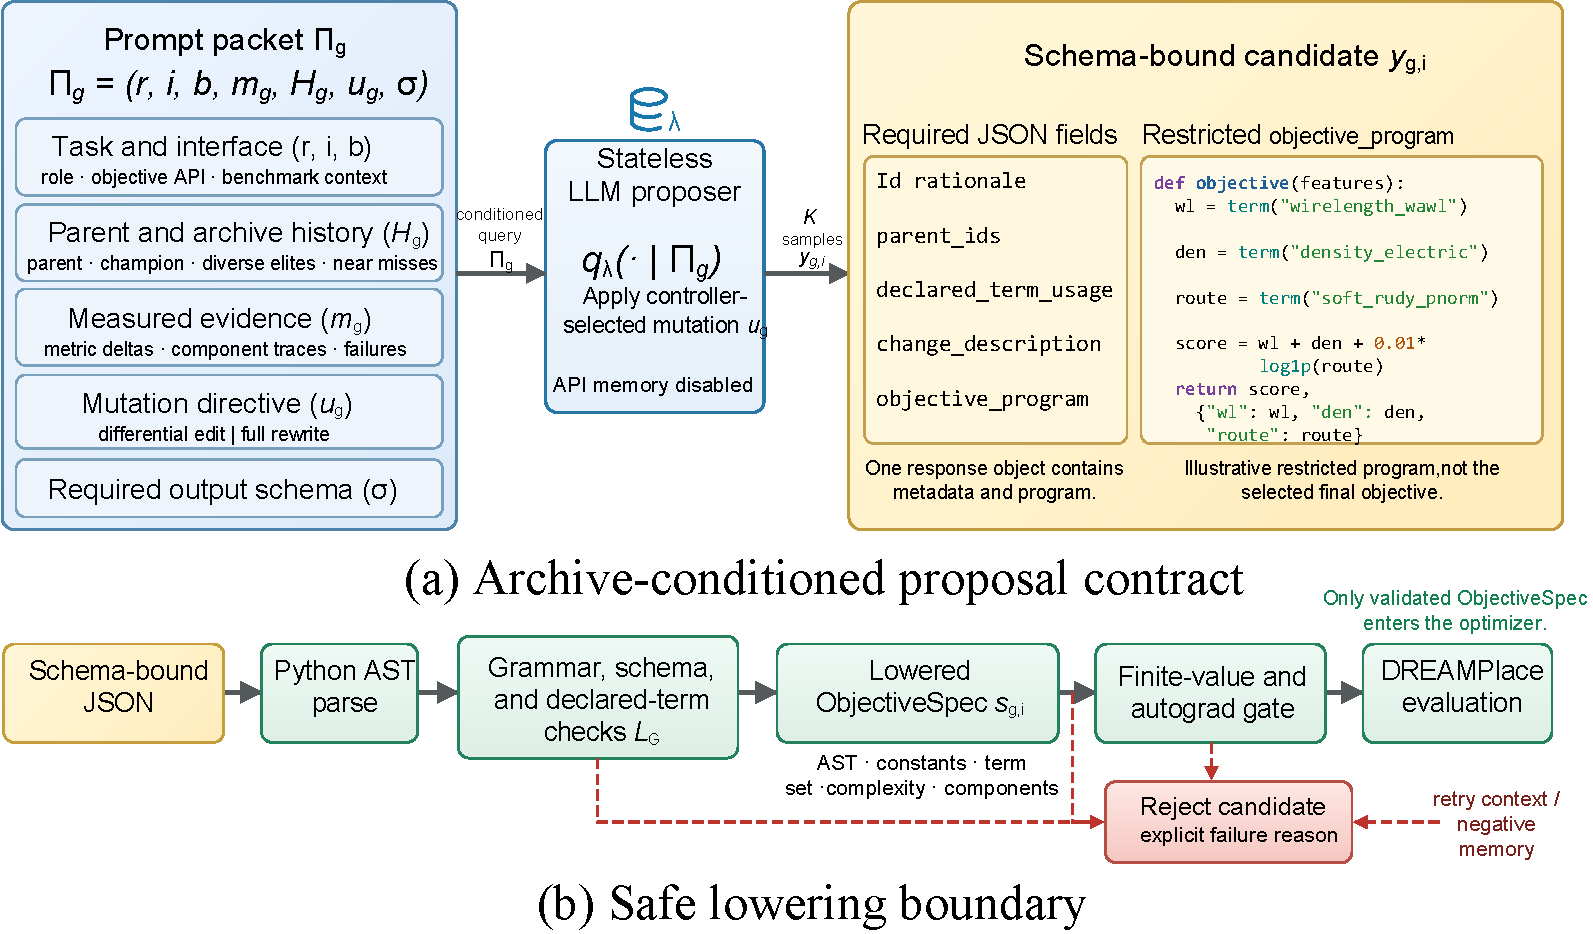
\includegraphics[width=\columnwidth]{graphs/Figure2.pdf}
\caption{Proposal and lowering contracts. (a) A fixed objective interface and
measured archive context condition $K$ stateless LLM samples. (b) Schema, AST,
term, and autograd checks lower a valid response into \texttt{ObjectiveSpec};
rejections return an explicit retry or negative-memory record.}
\Description{An archive-conditioned prompt supplies task, parent, measured
evidence, mutation, and schema context to a stateless LLM. A schema-bound
candidate is parsed and lowered into an ObjectiveSpec. Static or autograd
failures produce explicit rejection feedback, and only valid records reach
DREAMPlace.}
\label{fig:prompt-schema}
\end{figure}

\subsection{Safe Objective Lowering}
\label{sec:safe-interface}

The lowering boundary makes the model's action space finite. Static admission
validates JSON, parses the Python AST as data, checks declared against observed
terms, and lowers score and component expressions into \texttt{ObjectiveSpec}:
\begin{equation}
L_{\mathcal{G}}(y)=
\begin{cases}
s, & \mathrm{static}_{\mathcal{G}}(y)=1,\\
\bot, & \text{otherwise}.
\end{cases}
\label{eq:lowering-map}
\end{equation}
The grammar permits constants, local assignments, named \texttt{term} calls,
arithmetic, safe division, and \texttt{log1p}, \texttt{sqrt}, \texttt{square},
\texttt{softplus}, and \texttt{sigmoid}. It rejects control flow, imports,
arbitrary calls, mutation, randomness, and direct feature access. AST depth is
at most five, with 12 primitives per expression and six returned diagnostics.

Terms include weighted-average and log-sum-exp wirelength; electric and
bell-shaped density; soft-RUDY mean and hotspot pressure; and long-net,
pin-density, and pin-count-weighted pressure. Static compatibility requires
exactly one wirelength and one density family and rejects unavailable terms,
baseline clones, and out-of-range routing coefficients. Nonlinear interactions
remain expressible without duplicated anchors or ill-scaled objectives.

Dynamic admission occurs on the first DREAMPlace objective call. DREAMPlace
evaluates only the lowered AST, differentiates the resulting scalar, and
allows optimization to continue only when
\begin{equation}
\begin{aligned}
\mathcal{F}_{\mathrm{safe}}=\{f_s\mid{}&
\mathrm{terms}(f_s)\subseteq\mathcal{T},\quad
|f_s(\mathbf{x}_0)|<\infty,\\
&0<\|\nabla_{\mathbf{x}}f_s(\mathbf{x}_0)\|_2<\infty,\quad
\mathrm{compat}(f_s)=1\}.
\end{aligned}
\label{eq:safe-family}
\end{equation}
Runtime guards repeat finite checks throughout placement and terminate at the
first invalid state. The initial autograd gate establishes local executability;
the guards catch later instability. Raw model code is never imported or
executed.

\subsection{Cost-Scaled Evaluation}
\label{sec:cascade}
\label{sec:proxy-audit}

Expensive evidence is allocated only after optimizer compatibility. Tier~A
runs each admitted objective on a multi-design DREAMPlace panel and records
HPWL, density overflow, runtime, convergence, gradient behavior, per-design
outcomes, and component trajectories. Tier~B adds placement-RC timing when
collateral exists: search uses FLUTE/Elmore, while final WNS/TNS use OpenTimer
and are not called post-route timing. Tier~C routes scheduled promotions
through OpenROAD/ChiPBench and records global-route wirelength, routed
congestion or overflow, available post-GRT timing, runtime, and failure stage.

Tier~A first applies feasibility and robustness constraints. Let
$\bar g_H,\bar g_D$ denote mean HPWL and density-overflow gains,
$g_H^{\min},g_D^{\min}$ their worst-design gains, and $q_{HD}$ the fraction of
designs improving both metrics. The admission indicator is
\begin{equation}
\begin{aligned}
\chi_A(f)=\mathbb{I}\bigl[{}&
\bar g_H\geq-\delta_H,\quad \bar g_D\geq0,\\
&g_H^{\min}\geq-\delta_H^d,\quad
g_D^{\min}\geq-\delta_D^d,\\
&n_{\mathrm{struct}}=n_{\mathrm{severe}}=0\bigr],
\end{aligned}
\label{eq:parent-gate}
\end{equation}
where fixed tolerances admit bounded HPWL and per-design numerical noise. The
search score is
\begin{equation}
\begin{aligned}
S_A(f)=\chi_A(f)\biggl(&w_H[\bar g_H]_+ +w_D[\bar g_D]_+
+\frac{w_R}{1+\bar r_A(f)}\\
&+w_Qq_{HD}(f)-\eta c(f)\biggr),
\end{aligned}
\label{eq:selection-score}
\end{equation}
where $[z]_+=\max(z,0)$, $\bar r_A$ averages rank across design-seed cells, and
$c(f)$ is complexity. Weights and tolerances are fixed before a run. An elite
must also beat the same-flow fixed-objective portfolio and Pareto-improve over
its strongest HPWL/overflow member. Bounded distinct tradeoffs may enter
$\mathcal{P}_g$ as near misses but cannot become routed finalists before
passing the elite gate.

Cheap timing signals affect selection only when they add information beyond
HPWL. For timing delta $q\in\{\Delta\mathrm{WNS},\Delta\mathrm{TNS}\}$, the
perturbation audit computes
\begin{equation}
\rho_H(q)=\max\left\{
|\mathrm{Pearson}(\Delta\mathrm{HPWL},q)|,
|\mathrm{Spearman}(\Delta\mathrm{HPWL},q)|\right\}.
\label{eq:proxy-correlation}
\end{equation}
Let $a_C(q)$ indicate that held-out routed promotions preserve the proxy's rank
direction for the corresponding downstream timing metric. Its selection weight
is
\begin{equation}
\gamma_q=a_C(q)
\begin{cases}
0, & \rho_H(q)>0.95,\\
\gamma_{\mathrm{tie}}, & 0.70\leq\rho_H(q)\leq0.95,\\
\gamma_{\mathrm{soft}}, & \rho_H(q)<0.70,
\end{cases}
\quad 0<\gamma_{\mathrm{tie}}<\gamma_{\mathrm{soft}}\leq1.
\label{eq:proxy-admission}
\end{equation}
Until enough routed samples exist, $a_C(q)=0$ and timing remains diagnostic.
Low HPWL correlation establishes non-redundancy; routed agreement establishes
downstream relevance.

Every $\tau_C$ generations, at most $k_C$ unrouted elites are promoted while
$N_C<B_C$. The batch mixes high-$S_A$ candidates with strong occupants of
uncovered mechanism cells, then removes duplicate ASTs and signatures. Tier-C
results are committed before $\Pi_{g+1}$. The final score compares only
candidates with matched downstream evidence:
\begin{equation}
S_{\mathrm{final}}(f)=
\frac{1}{1+\bar r_C(f)}-\eta_Cc(f),
\label{eq:final-score}
\end{equation}
where $\bar r_C$ averages rank over reported post-GRT metrics and $\eta_Cc(f)$
favors compact objectives only when ranks tie.

\subsection{Archive and Closed-Loop Feedback}
\label{sec:archive}
\label{sec:search}

Each archive record contains parent, island, generation, prompt, provider
snapshot and decoding settings, raw response, lowered AST, terms, components,
complexity, tool configuration, per-design metrics, trajectories, artifacts,
and failure reason. Structural failures and completed regressions remain
queryable as negative memory but cannot occupy elite cells; near misses are
exploration-only.

MAP-Elites assigns each parent-eligible candidate to
\begin{equation}
\phi(f)=\bigl(b_{\mathrm{size}}(f),m(f),b_{\mathrm{hpwl}}(f),
b_{\mathrm{dens}}(f),b_{\mathrm{timing}}(f)\bigr),
\label{eq:archive-key}
\end{equation}
where $m(f)$ identifies wirelength-density, route-pressure, long-net,
pin-pressure, fanout-weighted, or hybrid mechanisms; missing timing maps to an
unknown bucket. Each island retains the strongest eligible program per cell:
\begin{equation}
\mathcal{A}_{g+1}[b]=
\arg\max_{u\in\mathcal{A}_g[b]\cup\{f\}}S_A(u),
\qquad b=\phi(f).
\label{eq:archive-update}
\end{equation}
Ring migration periodically copies eligible cell elites into neighboring
islands, where the same cell-replacement rule applies.

Feedback reconstruction converts tool records into compact, actionable
evidence:
\begin{equation}
\begin{aligned}
\mathbf{m}_{g+1}=\operatorname{Summarize}\bigl(&
\Delta\mathrm{rank},\Delta\mathrm{metric},
\mathbf{z}_{\mathrm{design}},\\
&\mathbf{z}_{\mathrm{comp}},\mathbf{z}_{\mathrm{fail}},
\mathbf{z}_{\mathrm{route}}\bigr).
\end{aligned}
\label{eq:feedback-summary}
\end{equation}
$\mathbf{z}_{\mathrm{design}}$ reports per-design and worst-case behavior.
$\mathbf{z}_{\mathrm{comp}}$ stores each component's start/mid/end, range,
mean, trend, and saturation status. $\mathbf{z}_{\mathrm{fail}}$ records
parser, gradient, convergence, and flow failures with repair lessons.
$\mathbf{z}_{\mathrm{route}}$ identifies which placement gains survive routing.
Equation~\eqref{eq:retrieval-policy} selects the programs that accompany this
scorecard in the next prompt.

CoEvoP\&R couples objective evolution to progressively updated placement and
routing evidence without training or mutating the EDA tools. Each routed
promotion can change parent selection, retrieval, or failure context.
Checkpointed prompts, responses, lowered records, metrics, and artifacts make
lineages auditable despite nondeterministic providers. Algorithm~\ref{alg:objective-evolution}
summarizes the loop.

\begin{algorithm}[t]
\caption{CoEvoP\&R objective evolution}
\label{alg:objective-evolution}
\scriptsize
\begin{algorithmic}[1]
\REQUIRE $\mathcal{G},\mathcal{D}_S,\mathcal{B}$;
$G,K,B_A,B_B,B_C,\tau_C,k_C,\tau_{\mathrm{mig}}$
\ENSURE Archive $\mathcal{A}_G$ and routed objective $f^*$
\STATE $\mathcal{A}_0\leftarrow\mathrm{EvaluateSeeds}(\mathcal{B},\mathcal{D}_S)$;
$N_A,N_B,N_C\leftarrow0$
\FOR{$g=0,\ldots,G-1$}
  \STATE $i\leftarrow g\bmod I$;
  $p_g\sim\pi_{\mathrm{par}}(\cdot\mid\mathcal{A}_g^{(i)})$
  \STATE $\mathcal{H}_g\leftarrow\mathrm{Retrieve}(\mathcal{A}_g,p_g)$;
  $u_g\leftarrow\mathrm{DiffOrRewrite}(\mathcal{A}_g,p_g)$
  \STATE $\Pi_g\leftarrow\mathrm{Prompt}(p_g,u_g,\mathbf{m}_g,\mathcal{H}_g)$;
  $\mathcal{Y}_g\leftarrow\{y_{g,j}\}_{j=1}^{K}\sim q_\lambda(\cdot\mid\Pi_g)$
  \FOR{$y\in\mathcal{Y}_g$}
    \STATE $s\leftarrow L_{\mathcal{G}}(y)$
    \IF{$s=\bot$}
      \STATE $\mathrm{RememberFailure}(y)$; \textbf{continue}
    \ENDIF
    \FOR{$f\in\mathrm{Calibrate}(s)$}
      \IF{$N_A\geq B_A$} \STATE \textbf{break} \ENDIF
      \STATE $\mathbf{m}_A\leftarrow E_A(f,\mathcal{D}_S)$; $N_A\leftarrow N_A+1$
      \STATE $\mathbf{m}_B\leftarrow\varnothing$; run $E_B(f)$ and increment $N_B$
      only if proxy-admitted and $N_B<B_B$
      \STATE $\mathcal{A}_g\leftarrow\mathrm{Insert}(\mathcal{A}_g,f,\mathbf{m}_A,\mathbf{m}_B)$
    \ENDFOR
  \ENDFOR
  \IF{$(g+1)\bmod\tau_C=0$ and $N_C<B_C$}
    \STATE $\mathcal{C}_g\leftarrow\mathrm{Promote}(\mathcal{A}_g,k_C,B_C-N_C)$
    \STATE $\mathbf{m}_C\leftarrow E_C(\mathcal{C}_g)$;
    $N_C\leftarrow N_C+|\mathcal{C}_g|$
    \STATE $\mathrm{CommitRoutedFeedback}(\mathcal{A}_g,\mathbf{m}_C)$
  \ENDIF
  \STATE $\mathcal{A}_{g+1}\leftarrow\mathrm{Migrate}(\mathcal{A}_g)$ if scheduled,
  else $\mathcal{A}_g$
\ENDFOR
\STATE \RETURN $\mathcal{A}_G,
f^*=\arg\max_{f\in\mathcal{A}^{C}_G}S_{\mathrm{final}}(f)$
\end{algorithmic}
\end{algorithm}


\begin{table*}[t]
\centering
\caption{Main results and intra-family transfer on ChiPBench Nangate45.
Values are mean improvements over native DREAMPlace across three seeds.
Within each panel and column, \colorbox{rankfirst}{\textbf{bold}} marks the
best result and \colorbox{ranksecond}{\underline{underline}} marks the
second-best result; ties share the best mark.}
\label{tab:chipbench-main}

\scriptsize
\renewcommand{\arraystretch}{1.02}
\setlength{\tabcolsep}{1.5pt}

% ---------- HPWL ----------
\begin{minipage}[t]{0.492\textwidth}
\centering
\textbf{(a) HPWL reduction (\%), $\uparrow$}\par
\vspace{2pt}

\begin{tabular*}{\linewidth}{
  @{\extracolsep{\fill}} l *{9}{r} @{}
}
\toprule
Method
& BP-FE & BP-BE & Swerv & Eth.
& DFT & OR1200 & VGA & Mor. & Mean \\
\midrule
DREAMPlace       & 0.0 & 0.0 & 0.0 & 0.0 & 0.0 & 0.0 & 0.0 & 0.0 & 0.0 \\
DP4.0-TD         & -5.3 & -1.7 & -3.9 & -0.4 & -1.8 & -4.6 & 0.3 & -2.1 & -2.4 \\
Best expert      & -2.4 & 3.7 & -0.8 & 1.9 & -1.2 & 2.6 & 4.1 & -2.3 & 0.7 \\
BO-DSL           & -0.7 & 3.8 & 1.2 & 4.6 & -0.3 & 2.9 & 5.7 & -0.4 & 2.1 \\
AutoDMP          & \cellcolor{ranksecond}\underline{7.8} & \cellcolor{rankfirst}\textbf{8.6} & 11.3 & 12.7 & 5.4 & \cellcolor{ranksecond}\underline{6.9} & 14.8 & 9.7 & 9.7 \\
EvoPlace         & 2.4 & 6.8 & 5.1 & 9.7 & 0.9 & 4.3 & 14.6 & 6.1 & 6.2 \\
LaMPlace         & -19.4 & -8.7 & 4.2 & -11.6 & 3.8 & -5.4 & -26.3 & -2.1 & -8.2 \\
\midrule
\textbf{CoEvoP\&R-E}
                 & \cellcolor{rankfirst}\textbf{8.4} & \cellcolor{ranksecond}\underline{7.6} & \cellcolor{rankfirst}\textbf{38.4} & \cellcolor{rankfirst}\textbf{17.8} & \cellcolor{rankfirst}\textbf{9.3} & \cellcolor{rankfirst}\textbf{7.2} & \cellcolor{rankfirst}\textbf{31.7} & \cellcolor{rankfirst}\textbf{14.6} & \cellcolor{rankfirst}\textbf{16.9} \\
\textbf{CoEvoP\&R-L}
                 & 6.2 & 5.7 & \cellcolor{ranksecond}\underline{32.1} & \cellcolor{ranksecond}\underline{13.4} & \cellcolor{ranksecond}\underline{7.1} & 5.4 & \cellcolor{ranksecond}\underline{24.6} & \cellcolor{ranksecond}\underline{11.2} & \cellcolor{ranksecond}\underline{13.2} \\
\bottomrule
\end{tabular*}
\end{minipage}
\hfill%
% ---------- CONGESTION ----------
\begin{minipage}[t]{0.492\textwidth}
\centering
\textbf{(b) Density-overflow reduction (\%), $\uparrow$}\par
\vspace{2pt}

\begin{tabular*}{\linewidth}{
  @{\extracolsep{\fill}} l *{9}{r} @{}
}
\toprule
Method
& BP-FE & BP-BE & Swerv & Eth.
& DFT & OR1200 & VGA & Mor. & Mean \\
\midrule
DREAMPlace       & 0.0 & 0.0 & 0.0 & 0.0 & 0.0 & 0.0 & 0.0 & 0.0 & 0.0 \\
DP4.0-TD         & -2.4 & 0.7 & -1.8 & -2.3 & -0.4 & -1.1 & 0.4 & -1.2 & -1.0 \\
Best expert      & 4.7 & 6.8 & 0.9 & 3.4 & 1.6 & 4.2 & 2.7 & 3.7 & 3.5 \\
BO-DSL           & 6.3 & 5.4 & 2.8 & 4.9 & 2.7 & 6.1 & 4.2 & 5.4 & 4.7 \\
AutoDMP          & 9.4 & 11.7 & 7.8 & 13.6 & 8.4 & 10.7 & 14.2 & 12.9 & 11.1 \\
EvoPlace         & 1.8 & 2.9 & -0.6 & 2.7 & 0.3 & 2.4 & 3.6 & 0.7 & 1.7 \\
LaMPlace         & 12.3 & 21.4 & 14.6 & \cellcolor{rankfirst}\textbf{18.7} & 9.8 & 17.2 & \cellcolor{rankfirst}\textbf{24.6} & 13.4 & 16.5 \\
\midrule
\textbf{CoEvoP\&R-E}
                 & \cellcolor{rankfirst}\textbf{48.6} & \cellcolor{rankfirst}\textbf{36.4} & \cellcolor{rankfirst}\textbf{71.8} & \cellcolor{ranksecond}\underline{15.4} & \cellcolor{rankfirst}\textbf{32.4} & \cellcolor{rankfirst}\textbf{47.3} & \cellcolor{ranksecond}\underline{18.9} & \cellcolor{rankfirst}\textbf{22.6} & \cellcolor{rankfirst}\textbf{36.7} \\
\textbf{CoEvoP\&R-L}
                 & \cellcolor{ranksecond}\underline{42.8} & \cellcolor{ranksecond}\underline{31.7} & \cellcolor{ranksecond}\underline{62.4} & 12.7 & \cellcolor{ranksecond}\underline{27.6} & \cellcolor{ranksecond}\underline{40.8} & 14.7 & \cellcolor{ranksecond}\underline{18.4} & \cellcolor{ranksecond}\underline{31.4} \\
\bottomrule
\end{tabular*}
\end{minipage}

\vspace{5pt}

% ---------- WNS ----------
\begin{minipage}[t]{0.492\textwidth}
\centering
\textbf{(c) WNS gain (ns), $\uparrow$}\par
\vspace{2pt}
\setlength{\tabcolsep}{0.5pt}

\begin{tabular*}{\linewidth}{
  @{\extracolsep{\fill}} l *{9}{r} @{}
}
\toprule
Method
& BP-FE & BP-BE & Swerv & Eth.
& DFT & OR1200 & VGA & Mor. & Mean \\
\midrule
DREAMPlace       & 0 & 0 & 0 & 0 & 0 & 0 & 0 & 0 & 0 \\
DP4.0-TD         & +0.51 & \cellcolor{ranksecond}\underline{+0.56} & +0.20 & +0.59 & +0.11 & +0.98 & +0.19 & +0.26 & +0.43 \\
Best expert      & -0.14 & -0.21 & -0.08 & -0.18 & -0.04 & -0.28 & -0.03 & -0.09 & -0.13 \\
BO-DSL           & -0.06 & +0.04 & -0.09 & -0.03 & +0.01 & -0.13 & +0.03 & -0.01 & -0.03 \\
AutoDMP          & +0.27 & +0.28 & +0.08 & +0.22 & +0.05 & +0.59 & +0.07 & +0.14 & +0.21 \\
EvoPlace         & +0.04 & +0.06 & -0.03 & +0.03 & +0.01 & +0.07 & -0.04 & +0.02 & +0.02 \\
LaMPlace         & \cellcolor{rankfirst}\textbf{+0.70} & \cellcolor{rankfirst}\textbf{+0.78} & \cellcolor{rankfirst}\textbf{+0.46} & \cellcolor{rankfirst}\textbf{+0.72} & +0.22 & \cellcolor{ranksecond}\underline{+1.26} & +0.34 & \cellcolor{rankfirst}\textbf{+0.42} & \cellcolor{ranksecond}\underline{+0.61} \\
\midrule
\textbf{CoEvoP\&R-E}
                 & \cellcolor{ranksecond}\underline{+0.62} & \cellcolor{rankfirst}\textbf{+0.78} & \cellcolor{ranksecond}\underline{+0.42} & \cellcolor{ranksecond}\underline{+0.62} & \cellcolor{rankfirst}\textbf{+0.52} & \cellcolor{rankfirst}\textbf{+1.48} & \cellcolor{rankfirst}\textbf{+0.87} & \cellcolor{ranksecond}\underline{+0.28} & \cellcolor{rankfirst}\textbf{+0.70} \\
\textbf{CoEvoP\&R-L}
                 & +0.46 & +0.54 & +0.32 & +0.44 & \cellcolor{ranksecond}\underline{+0.38} & +1.02 & \cellcolor{ranksecond}\underline{+0.58} & +0.21 & +0.49 \\
\bottomrule
\end{tabular*}
\end{minipage}
\hfill%
% ---------- TNS ----------
\begin{minipage}[t]{0.492\textwidth}
\centering
\textbf{(d) TNS gain (ns), $\uparrow$}\par
\vspace{2pt}
\setlength{\tabcolsep}{0.5pt}

\begin{tabular*}{\linewidth}{
  @{\extracolsep{\fill}} l *{9}{r} @{}
}
\toprule
Method
& BP-FE & BP-BE & Swerv & Eth.
& DFT & OR1200 & VGA & Mor. & Mean \\
\midrule
DREAMPlace       & 0 & 0 & 0 & 0 & 0 & 0 & 0 & 0 & 0 \\
DP4.0-TD         & \cellcolor{rankfirst}\textbf{+208} & +270 & +95 & \cellcolor{rankfirst}\textbf{+588} & \cellcolor{ranksecond}\underline{+74} & \cellcolor{rankfirst}\textbf{+1785} & +150 & +220 & +424 \\
Best expert      & -22.4 & -34.6 & -12.7 & -68.4 & -8.7 & -178.6 & -13.4 & -27.2 & -46 \\
BO-DSL           & -12.4 & +6.8 & -18.7 & -14.6 & +4.2 & -52.7 & +8.9 & -6.4 & -10.6 \\
AutoDMP          & +112 & +114 & +30 & +324 & +14 & +840 & +49 & +80 & +195 \\
EvoPlace         & +8.4 & +14.7 & -4.2 & +22.6 & +2.8 & +38.4 & -9.7 & +6.3 & +9.9 \\
LaMPlace         & +156 & +138 & +102 & +384 & +49 & +1190 & +84 & +145 & +281 \\
\midrule
\textbf{CoEvoP\&R-E}
                 & \cellcolor{ranksecond}\underline{+178} & \cellcolor{rankfirst}\textbf{+987} & \cellcolor{rankfirst}\textbf{+648} & \cellcolor{ranksecond}\underline{+495} & \cellcolor{rankfirst}\textbf{+108} & \cellcolor{ranksecond}\underline{+1520} & \cellcolor{rankfirst}\textbf{+2846} & \cellcolor{rankfirst}\textbf{+517} & \cellcolor{rankfirst}\textbf{+912} \\
\textbf{CoEvoP\&R-L}
                 & +128 & \cellcolor{ranksecond}\underline{+684} & \cellcolor{ranksecond}\underline{+467} & +348 & +72 & +1090 & \cellcolor{ranksecond}\underline{+1968} & \cellcolor{ranksecond}\underline{+347} & \cellcolor{ranksecond}\underline{+638} \\
\bottomrule
\end{tabular*}
\end{minipage}

\vspace{2pt}
\parbox{\textwidth}{\scriptsize
BP-FE and BP-BE denote black-parrot frontend and backend; DP4.0-TD denotes
DREAMPlace 4.0-TD.
E denotes target-design evolution; L denotes leave-one-design-out transfer.
Each value uses DREAMPlace as the reference; higher is better.
HPWL and density overflow use shared DREAMPlace reevaluation of each emitted
mixed-size placement; WNS and TNS are OpenTimer placement-RC deltas.
Baseline references: DREAMPlace and DREAMPlace 4.0-TD~\cite{dreamplace,dreamplace4};
BO-DSL uses TPE~\cite{tpe}; AutoDMP~\cite{autodmp};
EvoPlace~\cite{evoplace}; LaMPlace~\cite{lamplace}. Best expert uses hand-coded HPWL-density,
RUDY~\cite{rudy}, and pin-density terms.}

\end{table*}

\section{Experiments and Results}

\subsection{Experimental Setup}

The evaluation tests whether CoEvoP\&R improves placement and post-GRT
quality, transfers across benchmark families, depends on its safety/proxy/archive
mechanisms, and remains robust across LLM providers. The primary panel uses
the eight ChiPBench Nangate45 designs in
Table~\ref{tab:chipbench-main}~\cite{chipbench}: bp\_fe, bp\_be,
swerv\_wrapper, ethernet, dft68, or1200, vga\_lcd, and mor1kx.
Generalization uses ICCAD 2015 Superblue designs 1, 3, 4, 5, 7, 10, 16, and
18~\cite{iccad2015}, plus ASAP7 gcd, ibex, and ariane for zero-shot transfer
from Nangate45 to a 7-nm predictive process design kit~\cite{asap7}.

Baselines span analytical placement (DREAMPlace and DREAMPlace
4.0-TD~\cite{dreamplace,dreamplace4}), expert density/HPWL/RUDY/pin-density
objectives, same-grammar BO-DSL~\cite{tpe}, and shared-pipeline reruns of
AutoDMP~\cite{autodmp}, RoutePlacer~\cite{routeplacer},
EvoPlace~\cite{evoplace}, and LaMPlace~\cite{lamplace}.

Each method-design cell in Tables~\ref{tab:chipbench-main}
and~\ref{tab:generalization} uses three seeds with DREAMPlace as zero.
Table~\ref{tab:chipbench-main} reports DREAMPlace HPWL and density overflow plus
OpenTimer placement-RC WNS/TNS. Table~\ref{tab:generalization} reports post-GRT
wirelength, overflow, and OpenTimer timing.
A manifest keyed by design, method, seed, model, budgets, and metric records
objective hashes, prompts, artifacts, route status, and failures, making every
entry traceable. The default proposer is \texttt{gpt-5.4};
Section~\ref{sec:ablation} tests model-family sensitivity.

\subsection{Main Results on ChiPBench Nangate45}
\label{sec:main-results}

Table~\ref{tab:chipbench-main} combines target evolution and leave-one-design-out
(LODO) transfer. Every entry is a three-seed, same-flow rerun; DREAMPlace
provides HPWL/density overflow and OpenTimer provides placement-RC WNS/TNS.
Means aggregate design-seed cells, and higher is better. Target-specific and
LODO rows use distinct objectives. The Nangate45 champion reused
unchanged for cross-family transfer in Section~\ref{sec:generalization} is
\begin{equation}
f_{\mathrm{NG45}}(\mathbf{x})=\text{[Final formula]}.
\label{eq:final-objective}
\end{equation}

\begin{figure}[!ht]
\centering
\scriptsize
\setlength{\tabcolsep}{1pt}
\setlength{\fboxsep}{1pt}
\setlength{\fboxrule}{0.35pt}
\renewcommand{\arraystretch}{0.9}
\begin{tabular}{@{}cc@{}}
\begin{minipage}[t]{0.49\columnwidth}
\centering
\fbox{\begin{minipage}[c][0.405\columnwidth][c]{0.405\columnwidth}
\centering\tiny DREAMPlace\\placement + GRT-overflow overlay
\end{minipage}}

\textbf{(a) DREAMPlace}\\
HPWL=[F], GRT ovfl.=[F]\\
WNS=[F], TNS=[F]
\end{minipage}
&
\begin{minipage}[t]{0.49\columnwidth}
\centering
\fbox{\begin{minipage}[c][0.405\columnwidth][c]{0.405\columnwidth}
\centering\tiny DREAMPlace 4.0-TD\\placement + GRT-overflow overlay
\end{minipage}}

\textbf{(b) DREAMPlace 4.0-TD}\\
HPWL=[F], GRT ovfl.=[F]\\
WNS=[F], TNS=[F]
\end{minipage}
\\[0.45em]
\begin{minipage}[t]{0.49\columnwidth}
\centering
\fbox{\begin{minipage}[c][0.405\columnwidth][c]{0.405\columnwidth}
\centering\tiny Related baseline\\placement + GRT-overflow overlay
\end{minipage}}

\textbf{(c) Related baseline}\\
HPWL=[F], GRT ovfl.=[F]\\
WNS=[F], TNS=[F]
\end{minipage}
&
\begin{minipage}[t]{0.49\columnwidth}
\centering
\fbox{\begin{minipage}[c][0.405\columnwidth][c]{0.405\columnwidth}
\centering\tiny CoEvoP\&R\\placement + GRT-overflow overlay
\end{minipage}}

\textbf{(d) CoEvoP\&R}\\
HPWL=[F], GRT ovfl.=[F]\\
WNS=[F], TNS=[F]
\end{minipage}
\end{tabular}
\caption{Qualitative placement comparison on a representative hard design.
Each panel uses the same die outline, placement rendering, GRT-overflow
overlay, and color scale. The visual audit checks whether CoEvoP\&R's metric
gains correspond to reduced congestion artifacts while preserving layout structure.}
\Description{Four-panel qualitative placement comparison showing DREAMPlace,
DREAMPlace 4.0-TD, the strongest related baseline, and CoEvoP\&R with matching
placement and GRT-overflow overlays plus HPWL, GRT overflow, WNS, and TNS values.}
\label{fig:placement-qualitative}
\end{figure}

Figure~\ref{fig:placement-qualitative} compares a representative hard design
under identical placement and GRT-overflow rendering. Target evolution improves
mean HPWL/density overflow by
16.9\%/36.7\% versus best-baseline means of 9.7\%/16.5\%, and gains
0.70/912 ns WNS/TNS. LODO retains 13.2\%, 31.4\%, 0.49 ns, and 638 ns.

\begin{table}[!htbp]
\centering
\caption{Cross-family generalization on ICCAD 2015 Superblue and ASAP7.
All values are post-GRT improvements over DREAMPlace across three seeds.
DP4.0-TD abbreviates DREAMPlace 4.0-TD; rWL denotes OpenROAD global-route
wirelength. E denotes target-design evolution; T denotes zero-shot reuse of the
Nangate45 champion. Within each metric and circuit, \colorbox{rankfirst}{\textbf{bold}}
marks the best result and \colorbox{ranksecond}{\underline{underline}} marks
the second-best result; ties share the same rank. Higher is better.}
\label{tab:generalization}
\label{tab:asap7-transfer}
\scriptsize
\renewcommand{\arraystretch}{0.82}
\setlength{\tabcolsep}{1.0pt}
\resizebox{\columnwidth}{!}{%
\begin{tabular}{llccccccccccc}
\toprule
\multicolumn{2}{c}{} & \multicolumn{8}{c}{Superblue} & \multicolumn{3}{c}{ASAP7} \\
\cmidrule(lr){3-10}\cmidrule(lr){11-13}
Method & Metric & sb1 & sb3 & sb4 & sb5 & sb7 & sb10 & sb16 & sb18 & gcd & ibex & ariane \\
\midrule
\multirow{4}{*}{DREAMPlace}
  & rWL (\%)         & 0.0 & 0.0 & 0.0 & 0.0 & 0.0 & 0.0 & 0.0 & 0.0 & 0.0 & 0.0 & 0.0 \\
  & Cong.\ (\%)      & 0.0 & 0.0 & 0.0 & 0.0 & 0.0 & 0.0 & 0.0 & 0.0 & 0.0 & 0.0 & 0.0 \\
  & WNS ($\Delta$ns) & 0.0 & 0.0 & 0.0 & 0.0 & 0.0 & 0.0 & 0.0 & 0.0 & 0.0 & 0.0 & 0.0 \\
  & TNS ($\Delta$ns) & 0.0 & 0.0 & 0.0 & 0.0 & 0.0 & 0.0 & 0.0 & 0.0 & 0.0 & 0.0 & 0.0 \\
\midrule
\multirow{4}{*}{DP4.0-TD}
  & rWL (\%)         & -0.4 & -0.6 & +0.2 & -0.8 & -0.3 & +0.1 & -0.5 & +0.3 & +0.4 & -0.3 & -0.8 \\
  & Cong.\ (\%)      & +0.2 & -0.3 & -0.4 & +0.1 & -0.2 & -0.7 & -0.1 & +0.4 & +0.6 & +0.2 & -0.4 \\
  & WNS ($\Delta$ns) & \cellcolor{ranksecond}\underline{+4.4} & \cellcolor{rankfirst}\textbf{+16.8} & \cellcolor{ranksecond}\underline{+8.7} & \cellcolor{rankfirst}\textbf{+21.7} & \cellcolor{ranksecond}\underline{+5.2} & \cellcolor{ranksecond}\underline{+1.9} & \cellcolor{ranksecond}\underline{+4.7} & \cellcolor{rankfirst}\textbf{+8.3} & +0.06 & +0.18 & \cellcolor{ranksecond}\underline{+0.34} \\
  & TNS ($\Delta$ns) & \cellcolor{ranksecond}\underline{+16700} & +3370 & +5210 & +11300 & +9810 & \cellcolor{ranksecond}\underline{+7040} & \cellcolor{rankfirst}\textbf{+31400} & +4320 & +32 & +187 & \cellcolor{ranksecond}\underline{+584} \\
\midrule
\multirow{4}{*}{RoutePlacer}
  & rWL (\%)         & +0.1 & -0.3 & +0.1 & +0.3 & -0.1 & +0.9 & -0.1 & +0.2 & +0.4 & -0.6 & +1.8 \\
  & Cong.\ (\%)      & +3.1 & +1.7 & +4.6 & +3.9 & +3.9 & \cellcolor{rankfirst}\textbf{+43.2} & +1.4 & +3.7 & \cellcolor{ranksecond}\underline{+6.4} & \cellcolor{ranksecond}\underline{+18.7} & \cellcolor{ranksecond}\underline{+24.6} \\
  & WNS ($\Delta$ns) & -0.6 & -0.4 & +0.2 & -0.4 & -0.8 & -1.2 & -0.3 & -0.7 & -0.02 & -0.14 & -0.34 \\
  & TNS ($\Delta$ns) & -1400 & -800 & +200 & -1200 & -1600 & -3400 & -800 & -1400 & -12 & -87 & -294 \\
\midrule
\multirow{4}{*}{EvoPlace}
  & rWL (\%)         & -2.4 & -3.6 & +0.4 & -2.8 & +1.4 & -3.2 & -1.8 & +0.6 & +1.2 & -8.4 & -13.4 \\
  & Cong.\ (\%)      & -3.4 & -8.6 & -2.4 & -4.2 & +0.4 & -12.4 & -6.8 & -1.2 & +0.4 & -14.2 & -18.4 \\
  & WNS ($\Delta$ns) & +0.2 & +0.4 & +0.4 & -0.4 & +0.6 & -0.8 & -0.4 & +0.4 & +0.02 & -0.24 & -0.48 \\
  & TNS ($\Delta$ns) & -600 & -1400 & +400 & -1200 & +300 & -2200 & -1400 & +200 & +4 & -124 & -487 \\
\midrule
\multirow{4}{*}{LaMPlace}
  & rWL (\%)         & -4.6 & -6.8 & \cellcolor{rankfirst}\textbf{+14.2} & -8.4 & +0.4 & -2.4 & \cellcolor{rankfirst}\textbf{+11.8} & \cellcolor{rankfirst}\textbf{+22.4} & -6.8 & -18.4 & -22.4 \\
  & Cong.\ (\%)      & \cellcolor{ranksecond}\underline{+18.4} & +14.6 & \cellcolor{rankfirst}\textbf{+42.4} & +15.8 & \cellcolor{ranksecond}\underline{+19.4} & +20.6 & \cellcolor{rankfirst}\textbf{+48.6} & \cellcolor{rankfirst}\textbf{+32.4} & +2.4 & -8.7 & -14.2 \\
  & WNS ($\Delta$ns) & +2.4 & +6.8 & +3.4 & +8.4 & +3.6 & +1.2 & +2.8 & +0.4 & +0.04 & -0.16 & -0.32 \\
  & TNS ($\Delta$ns) & +2400 & +6800 & +2400 & +8400 & +3800 & +1400 & +1800 & +1200 & -18 & -94 & -246 \\
\midrule
\multirow{4}{*}{CoEvoP\&R-E}
  & rWL (\%)         & \cellcolor{rankfirst}\textbf{+5.4} & \cellcolor{rankfirst}\textbf{+6.2} & \cellcolor{ranksecond}\underline{+4.8} & \cellcolor{rankfirst}\textbf{+7.2} & \cellcolor{rankfirst}\textbf{+5.4} & \cellcolor{rankfirst}\textbf{+3.6} & \cellcolor{ranksecond}\underline{+6.4} & \cellcolor{ranksecond}\underline{+4.2} & \cellcolor{rankfirst}\textbf{+5.4} & \cellcolor{rankfirst}\textbf{+8.2} & \cellcolor{rankfirst}\textbf{+10.6} \\
  & Cong.\ (\%)      & \cellcolor{rankfirst}\textbf{+26.4} & \cellcolor{rankfirst}\textbf{+19.4} & \cellcolor{ranksecond}\underline{+22.6} & \cellcolor{rankfirst}\textbf{+22.4} & \cellcolor{rankfirst}\textbf{+21.7} & \cellcolor{ranksecond}\underline{+34.7} & \cellcolor{ranksecond}\underline{+9.8} & \cellcolor{ranksecond}\underline{+28.4} & \cellcolor{rankfirst}\textbf{+14.6} & \cellcolor{rankfirst}\textbf{+22.4} & \cellcolor{rankfirst}\textbf{+26.8} \\
  & WNS ($\Delta$ns) & \cellcolor{rankfirst}\textbf{+5.8} & \cellcolor{ranksecond}\underline{+14.8} & \cellcolor{rankfirst}\textbf{+9.4} & \cellcolor{ranksecond}\underline{+12.8} & \cellcolor{rankfirst}\textbf{+7.6} & \cellcolor{rankfirst}\textbf{+2.6} & \cellcolor{rankfirst}\textbf{+6.2} & \cellcolor{ranksecond}\underline{+6.4} & \cellcolor{rankfirst}\textbf{+0.24} & \cellcolor{rankfirst}\textbf{+0.42} & \cellcolor{rankfirst}\textbf{+0.68} \\
  & TNS ($\Delta$ns) & \cellcolor{rankfirst}\textbf{+18800} & \cellcolor{rankfirst}\textbf{+38400} & \cellcolor{rankfirst}\textbf{+18700} & \cellcolor{rankfirst}\textbf{+67200} & \cellcolor{rankfirst}\textbf{+36400} & \cellcolor{rankfirst}\textbf{+8400} & \cellcolor{ranksecond}\underline{+14600} & \cellcolor{rankfirst}\textbf{+6800} & \cellcolor{rankfirst}\textbf{+148} & \cellcolor{rankfirst}\textbf{+468} & \cellcolor{rankfirst}\textbf{+824} \\
\midrule
\multirow{4}{*}{CoEvoP\&R-T}
  & rWL (\%)         & \cellcolor{ranksecond}\underline{+1.4} & \cellcolor{ranksecond}\underline{+3.8} & +2.6 & \cellcolor{ranksecond}\underline{+4.2} & \cellcolor{ranksecond}\underline{+3.2} & \cellcolor{ranksecond}\underline{+1.8} & +3.6 & +2.4 & \cellcolor{ranksecond}\underline{+2.4} & \cellcolor{ranksecond}\underline{+3.8} & \cellcolor{ranksecond}\underline{+5.2} \\
  & Cong.\ (\%)      & +12.4 & \cellcolor{ranksecond}\underline{+14.8} & +14.6 & \cellcolor{ranksecond}\underline{+18.7} & +15.4 & +22.8 & +7.8 & +19.4 & \cellcolor{ranksecond}\underline{+6.4} & +11.8 & +14.6 \\
  & WNS ($\Delta$ns) & +1.4 & +8.2 & +5.4 & +7.4 & +4.6 & +1.8 & +4.6 & +4.2 & \cellcolor{ranksecond}\underline{+0.08} & \cellcolor{ranksecond}\underline{+0.22} & \cellcolor{ranksecond}\underline{+0.34} \\
  & TNS ($\Delta$ns) & +2400 & \cellcolor{ranksecond}\underline{+18400} & \cellcolor{ranksecond}\underline{+9600} & \cellcolor{ranksecond}\underline{+32400} & \cellcolor{ranksecond}\underline{+14200} & +4800 & +7600 & \cellcolor{ranksecond}\underline{+4600} & \cellcolor{ranksecond}\underline{+58} & \cellcolor{ranksecond}\underline{+204} & +368 \\
\bottomrule
\end{tabular}
}
\vspace{1pt}
\parbox{\columnwidth}{\scriptsize
All rows use the shared OpenROAD post-GRT flow. rWL is global-route
wirelength, Cong.\ is total global-routing overflow reduction, and WNS/TNS
come from OpenTimer on the post-GRT routed netlist.
Baseline references follow Table~\ref{tab:chipbench-main}: DREAMPlace and
DREAMPlace 4.0-TD~\cite{dreamplace,dreamplace4};
RoutePlacer~\cite{routeplacer}; EvoPlace~\cite{evoplace};
LaMPlace~\cite{lamplace}. All tabulated values are shared-pipeline reruns.
LaMPlace publishes Innovus post-detail-route results for superblue4,
superblue16, and superblue18; those values provide a directional, not
numerically equivalent, comparison to our post-GRT flow.}
\end{table}

\subsection{Generalization}
\label{sec:generalization}

Table~\ref{tab:chipbench-main} measures intra-family LODO; Table~\ref{tab:generalization}
compares target-design evolution (E) with zero-shot reuse of the exact
Nangate45 objective (T) on Superblue and ASAP7. Target metrics are excluded
from transfer prompts and parent selection.

On Superblue, E averages 5.4\% rWL, 23.2\% GRT-overflow reduction, 8.2 ns WNS,
and 26,163 ns TNS gain. T retains 2.9\%, 15.7\%, 4.7 ns, and 11,750 ns,
respectively, or 45\%--68\% of E. LaMPlace leads E in rWL and congestion on
superblue4/16/18, while DP4.0-TD leads TNS on superblue16. On ASAP7,
LaMPlace regresses while both CoEvoP\&R variants remain positive, supporting
symbolic cross-node transfer. Superblue1 is the clearest transfer-limit case.

\subsection{Proxy Audit}

\begin{table}[!htbp]
\caption{Timing-proxy admission audit on the four-design stress panel.
Perturbations use 100, 250, 500, 1000, and 2000 DBU. Thresholds follow
Section~\ref{sec:proxy-audit}; Influence reports the policy after the routed
agreement gate.}
\label{tab:proxy-audit}
\centering
\scriptsize
\setlength{\tabcolsep}{1.5pt}
\resizebox{\columnwidth}{!}{%
\begin{tabular}{lcccc}
\toprule
Metric pair & Med.\ Pearson & Med.\ Spearman & A/T/R & Influence \\
\midrule
$\Delta$WNS vs.\ $\Delta$HPWL & 0.58 & 0.54 & 3/1/0 & soft gate \\
$\Delta$TNS vs.\ $\Delta$HPWL & 0.82 & 0.78 & 1/2/1 & tie-breaker \\
\bottomrule
\end{tabular}
}
\end{table}

Table~\ref{tab:proxy-audit} reports Pearson/Spearman correlation and
admitted/tie-weighted/rejected counts (A/T/R) on bp\_fe, swerv, ethernet, and
ariane133. These correlations test HPWL non-redundancy; held-out agreement with
subsequent Tier-C timing determines whether the indicated weight is activated.
The ungated timing-proxy control tests this two-part policy.

\subsection{Causal Controls and Model Sensitivity}
\label{sec:ablation}

\begin{table}[!htbp]
\caption{Claim-aligned controls and model robustness on the four-design stress
panel. Proposal and archive controls match candidate and Tier-C budgets; direct
Tier~C routes every valid candidate. Valid/Acc.: valid/accepted objectives;
H/D: HPWL/density-overflow reduction; W/T: WNS/TNS gain. Score follows
Equation~\eqref{eq:selection-score}; Cost is total GPU-hours.}
\label{tab:ablation-efficiency}
\centering
\scriptsize
\setlength{\tabcolsep}{1.5pt}
\renewcommand{\arraystretch}{0.88}
\resizebox{\columnwidth}{!}{%
\begin{tabular}{p{0.34\columnwidth}cccccc}
\toprule
Configuration & Valid/Acc. & Score & H/D & W/T & Tier-C & Cost \\
& & & (\%) & ($\Delta$ns) & evals & (GPU-h) \\
\midrule
\textbf{Full CoEvoP\&R} & 68/12 & 4.87 & 18.4/42.6 & +0.68/+624 & 24 & 84 \\
\midrule
\multicolumn{7}{l}{\textit{Proposal: objective-search policy}} \\
Random DSL evolution       & 42/4  & 1.24 & 2.4/4.8   & +0.08/+42  & 24 & 68 \\
One-shot LLM sampling      & 58/8  & 2.14 & 6.4/12.4  & +0.24/+184 & 24 & 42 \\
Score-only LLM evolution   & 62/10 & 3.42 & 12.6/24.8 & +0.42/+318 & 24 & 76 \\
\midrule
\multicolumn{7}{l}{\textit{Evaluation: interface and evidence policy}} \\
Prompt-only free-form interface & 24/4  & 1.86 & 5.4/11.4  & +0.16/+112 & 24 & 72 \\
Tier-A-only selection      & 68/18 & 2.68 & 8.4/14.6  & +0.24/+186 & 0  & 12 \\
Direct Tier C (all valid)  & 68/8  & 3.14 & 10.6/22.4 & +0.34/+348 & 68 & 168 \\
Ungated timing proxy       & 68/14 & 3.86 & 14.8/32.6 & +0.48/+412 & 24 & 86 \\
\midrule
\multicolumn{7}{l}{\textit{Archive: retained search state}} \\
Champion-only scalar history & 62/10 & 2.42 & 8.6/16.4  & +0.28/+218 & 24 & 82 \\
Top-$k$ scalar archive       & 64/11 & 3.14 & 12.4/24.8 & +0.38/+312 & 24 & 84 \\
MAP-Elites, metrics only     & 66/12 & 3.68 & 15.2/32.4 & +0.48/+412 & 24 & 84 \\
\midrule
\multicolumn{7}{l}{\textit{Model-family sensitivity}} \\
\texttt{gpt-5.4} (default)    & 68/12 & 4.87 & 18.4/42.6 & +0.68/+624 & 24 & 84 \\
\texttt{gpt-4.1-mini}         & 62/10 & 3.87 & 14.8/34.2 & +0.52/+468 & 24 & 68 \\
\texttt{claude-opus-4-8}      & 66/12 & 4.62 & 17.4/40.8 & +0.64/+584 & 24 & 92 \\
\texttt{qwen3.7-max}          & 58/9  & 3.24 & 12.6/26.8 & +0.44/+368 & 24 & 74 \\
\bottomrule
\end{tabular}
}
\end{table}

Table~\ref{tab:ablation-efficiency} asks one causal question per stage of
Figure~\ref{fig:loop}. Proposal controls separate the LLM prior, iterative search,
and execution feedback through random DSL evolution, equal-sample one-shot
generation, and score-only evolution. Evaluation controls compare the
machine-checkable interface against prompt-only free-form proposals, Tier-A-only
selection, routing every valid candidate at Tier~C, and an ungated timing proxy.
Every row sends only lowered, autograd-valid objectives to DREAMPlace; raw
proposals remain data.

Archive controls compare champion-only scalars, top-$k$ scalar history, and a
metrics-only MAP-Elites archive against full feedback reconstruction. Proposal
and archive rows match candidate and Tier-C budgets. Model rows hold prompts,
mutation schedules, and evaluator
budgets fixed while comparing the default proposer, an efficient same-provider
model, and frontier models from Anthropic and Qwen. These controls attribute
performance to proposal search, evidence allocation, and retained execution
state.


\section{Conclusion}

CoEvoP\&R turns routing-aware placement-objective design into a search over
complete executable replacement objectives. The framework combines a safe
objective interface, cost-scaled placement and routing evaluation, proxy
admission, and a routed-feedback archive loop.
These components let
LLM-generated objectives enter analytical placement without arbitrary code
execution or unchecked proxy feedback.

Across eight ChiPBench Nangate45 designs, target-evolved objectives reduce
HPWL by 16.9\% and density overflow by 36.7\% over native DREAMPlace while
improving OpenTimer placement-RC WNS by 0.70 ns and TNS by 912 ns. LODO
transfer retains 13.2\% HPWL reduction, 31.4\% density-overflow reduction,
0.49 ns WNS gain, and 638 ns TNS gain. Superblue and ASAP7 results further
measure target-design evolution and zero-shot cross-family transfer under a
shared post-GRT flow.

CoEvoP\&R gives EDA objective design a measured search interface. Many
physical-design loops rely on cheap proxy signals while optimizing for
expensive downstream costs. CoEvoP\&R evolves symbolic objectives under that
hierarchy while keeping optimizer execution fail-closed and proxy influence
auditable.



\bibliographystyle{ACM-Reference-Format}
\bibliography{sample-base}

\end{document}
